\chapter{Genomic prediction: a brief overview}

Let's review the basic approach we use in genome-wide association
mapping.

\begin{itemize}

\item We measure both the phenotype, $y_i$, of individual $i$ and its
  genotype at a large number of loci, where $x_{ij}$ is the
  individual's genotype at locus $j$.

\item We regress phenotype on genotype one locus at a time, using a
  random effect to correct for phenotypic similarities that reflect
  relatedness rather than similarity in genotype. 
\[
y_i^{(k)} = x_{ij}\beta_j + \phi^{(k)} + \epsilon_i \quad .
\]

\end{itemize}

Keep in mind this is a highly idealized schematic of how GWAS analyses
are actually done.\footnote{Remember, also, that in analyses of human
  disease, a case-control approach is often used rather than the
  regression approach I've been focusing on.} If you want to do GWAS
for real, you should take a look at
GEMMA~(\url{http://www.xzlab.org/software.html})\index{GEMMA} or
TASSEL~(\url{https://www.maizegenetics.net/tassel}).\index{TASSEL} One
important way in which what I've presented is a simplification is that
in a real GWAS analysis, you'd estimate the effects of every locus
simultaneously, which raises an interesting problem.

In a typical GWAS analysis\footnote{In humans at least}, you will have
measured the phenotype of a few thousand individuals, but you will
have genotyped those individuals at several hundred thousand
loci. Lango Allen et al.~\cite{LangoAllen-etal-2010}, for example,
report results from a large analysis of height variation in humans,
183,727 individuals genotyped at 2,834,208 loci. What's the problem
here?

There are more predictors~(loci) than observations~(individual
phenotypes). If you remember some basic algebra, you'll remember that
you can't solve a set of linear equations unless you have the same
number of equations as unknowns. For example, you can't solve a set of
three equations that has five unknowns. There's a similar phenomenon
in statistics when we're fitting a linear regression. In statistics we
don't ``solve'' an equation. We find the best fit in a regression, and
we can do so in a reasonable way so long as the number of observations
exceeds the number of variables included in our regression. To put a
little mathematical notation to it, if $n$ is the number of
observations and $p$ is the number of regression parameters we hope to
estimate, life is good (meaning that we can estimate the regression
parameters) so long as $n > p$.\footnote{And the more that $n$ exceeds
  $p$ the better, the more accurate our estimates of the regression
  parameters will be.} The typical situation we encounter in GWAS is
that $n < p$, which means we have to be really sneaky. Essentially
what we do is that we find a way for the data to tell us that a lot of
the parameters don't matter and we fit a regression only to the ones
that do, {\it and\/} we set things up so that the remaining number of
parameters is less than $n$. If that all sounds a little hoky, trust
me it isn't. There are good ways to do it and good statistical
justification for doing it\footnote{And biological justification for
  doing it in GWAS.}, but the mathematics behind it gets pretty hairy,
which is why you want to use GEMMA or TASSEL for a real GWAS. We'll
ignore this part of the challenge associated with GWAS and focus on
another one: complex traits often are influenced by a very large
nubmer of loci. That is, after all, why we started studying
quantitative genetics in the first place.

\section*{Genetics of complex traits}

Let's return to that Lango Allen et al.~\cite{LangoAllen-etal-2010}
GWAS on height in humans. They identified at least 180 loci associated
with differences in height. Moreover, many of the variants are closely
associated with genes that are part of previously identified pathways,
e.g., Hedgehog signaling,\footnote{``The Hedgehog signaling pathway is
  a signaling pathway that transmits information to embryonic cells
  required for proper cell differentiation.''
  \url{https://en.wikipedia.org/wiki/Hedgehog_signaling_pathway},
  accessed 14 August 2021.} or
that were previously identified as being involved in skeletal growth
defects. A more recent study by Wood et al.~\cite{Wood-etal-2014}
synthesized results from 79 studies involving 253,288 individuals and
identified 697 variants that were clustered into 423 loci affecting
differences in height.\footnote{It's worth noting that even this is
  likely to be an underestimate of the number of loci associated with
  height variation in humans because all of the individuals included
  in the analysis were of European ancestry.} Think about what that
means. If you know my genotype at only one of those 697 variants, you
know next to nothing about how tall I am. But what if you knew my
genotype for all of those variants? Then you should be able to do
better.\index{Genome-wide association study!human height}

The basic idea is fairly simple. When you do a full GWAS and estimate
the effects at every locus simultaneously, you are essentially
performing a multiple regression of phenotype on all of the loci
you've scored simultaenously instead of looking at them one at a
time. In equation-speak,
\[
y_i^{(k)} = \sum_j x_{ij}\beta_j + \phi^{(k)} + \epsilon_i \quad .
\]
Now think a bit more about what that equation means. The $\phi^{(k)}$
and $\epsilon_i$ terms represent random variation, in the first case
variation that is correlated among individuals depending on how
closely related they are and in the second case variation that is
purely random. The term $\sum_j x_{ij}\beta_j$ reflects systematic
effects associated with the genotype of individual $i$. In other
words, if we know individual $i$'s genotype, i.e., if we know $x_{ij}$
we can predict what phenotype it will have, namely
$\mu_i = \sum_j x_{ij}\beta_j$. Although we know there will be
uncertainty associated with this prediction, $\mu_i$ is our best guess
of the phenotype for that individual, i.e., our genomic prediction or
polygenic score. In the case of height in human beings, it turns out
that the loci identified in Wood et al.~\cite{Wood-etal-2014} account
for about 16 percent of variation in height.\footnote{In Europe the
  heritability of height at age 20 is about 80
  percent~\cite{Jelenkovic-etal-2016}.}\index{genomic predictioon}
\index{polygenic score} If we don't have too many groups, we could
refine our estimate a bit further by adding in the group-specific
estimate, $\phi^{(k)}$. Of course when we do so, our prediction is no
longer a {\it genomic\/} predictiion, {\it per se}. It's a genomic
prediction enhanced by non-genetic group information.

\subsection*{A toy example}

To make all of this more concrete, we'll explore a toy example using
the highly simplified one locus at a time approach to GWAS with a
highly simplified example of the multiple regression approach to
GWAS. You'll find an {\tt R} notebook that implements all of these
analyses at
\url{http://darwin.eeb.uconn.edu/eeb348-notes/Exploring-genomic-prediction.nb.html}. I
encourage you to download the notebook as you follow along. You will
find it especially useful if you try some different scenarios by
changing {\tt nloci} and {\tt effect} when you generate the data that
you later analyze locus by locus or with genomic prediction. Here's
what the code as written does:

\begin{itemize}

\item Generate a random dataset with 100 individuals and 20 loci, 5 of
  which influence the phenotype. The effect of one ``1'' allele at
  locus 1 is 1, at locus 2 -1, at locus 3 0.5, at locus 4 -0.5, and at
  locus 5 0.25. The standard deviation of the phenotype around the
  predicted mean is 0.2.

\item Run the locus-by-locus regression for each locus and store the
  results (mean and 95\% credible interval) in {\tt results}. {\tt
    results} is sorted in by the magnitude of the posterior mean, so
  that loci with the largest estimated effect occur at the top and
  loci with the smallest effect occur at the bottom.

\item Run the multiple regression and store the results in {\tt
    results\_gp}.  
    
\end{itemize}

If you look at the code, you'll see that I use {\tt stan\_lm()} rather
than using {\tt stan\_lmer()}. That's because I simulate the data without
family structure, so there's no need to include the family random
effect.

Table~\ref{table:single} shows results of the locus by locus analysis.

\begin{table}
  \centering
\begin{tabular}{rrrr}
  \hline
 & mean & 2.5\% & 97.5\% \\ 
  \hline
locus\_2  & -0.939 & -1.185 & -0.695 \\
locus\_1  & 0.747  & 0.491  & 0.951 \\
locus\_3  & 0.395  & 0.097  & 0.696 \\
locus\_15 & 0.312  & 0.031  & 0.587 \\
locus\_4  & -0.206 & -0.497 & 0.086 \\
locus\_11 & -0.182 & -0.494 & 0.136 \\
locus\_7  & -0.149 & -0.445 & 0.136 \\
locus\_12 & -0.123 & -0.439 & 0.176 \\
locus\_6  & -0.102 & -0.362 & 0.169 \\
locus\_19 & -0.086 & -0.379 & 0.214 \\
locus\_13 & -0.073 & -0.369 & 0.229 \\
locus\_17 & -0.072 & -0.397 & 0.264 \\
locus\_14 & 0.068  & -0.230 & 0.359 \\
locus\_10 & -0.065 & -0.334 & 0.208 \\
locus\_20 & -0.053 & -0.334 & 0.231 \\
locus\_18 & 0.040  & -0.261 & 0.337 \\
locus\_8  & 0.017  & -0.257 & 0.309 \\
locus\_9  & -0.010 & -0.310 & 0.302 \\
locus\_16 & -0.006 & -0.275 & 0.274 \\
locus\_5  & -0.005 & -0.315 & 0.28 \\
  \hline
\end{tabular}
\caption{Sample results for locus by locus analysis of genetic
  associations using {\tt genomic-prediction.R}}\label{table:single}
\end{table}

For this simulated data set 4 of the 5 loci with the largest estimated
effect are the 5 loci for which I specified an effect, one of them
(locus 15) did not have a specified effect and locus 5, which had a
specified effect, has the lowest estimated effect of all. 

What about the multiple regression approach? First, take a look at the
estimated effects~(Table~\ref{table:multiple}). Not only does this
approach pick out the right loci, the first five, none of the other
loci have particularly large estimated effects. The largest, {\tt
  locus\_17} is only about 0.07, about the same as in the locus by
locus analysis. It would take much more extensive simulation to
demonstrate the advantage empirically, but it is clear from first
principles that multiple regression analyses will be more reliable
than locus by locus analyses because a multiple regression analysis
takes account of random associations among loci.

\begin{table}
\centering
\begin{tabular}{rrrr}
  \hline
 & mean & 2.5\% & 97.5\% \\ 
  \hline
locus\_1  & 0.979  & 0.840  & 1.116 \\
locus\_2  & -0.882 & -1.016 & -0.742 \\
locus\_3  & 0.614 &  0.465  & 0.762 \\
locus\_4  & -0.514 & -0.656 & -0.373 \\
locus\_5  & 0.246  & 0.086  & 0.389 \\
locus\_17 & -0.070 & -0.217 & 0.028 \\
locus\_7  & -0.058 & -0.198 & 0.031 \\
locus\_18 & 0.053  & -0.037 & 0.196 \\
locus\_6  & 0.052  & -0.030 & 0.176 \\
locus\_8  & 0.042  & -0.037 & 0.159 \\
locus\_16 & 0.039  & -0.038 & 0.156 \\
locus\_10 & -0.034 & -0.147 & 0.044 \\
locus\_9  & 0.013  & -0.076 & 0.126 \\
locus\_11 & -0.010 & -0.119 & 0.082 \\
locus\_15 & 0.006  & -0.080 & 0.107 \\
locus\_12 & 0.005  & -0.086 & 0.106 \\
locus\_19 & -0.005 & -0.104 & 0.083 \\
locus\_20 & 0.003  & -0.082 & 0.095 \\
locus\_13 & -0.001 & -0.093 & 0.086 \\
locus\_14 & 0.001  & -0.091 & 0.093 \\
  \hline
\end{tabular}
\caption{Results from multiple regression analysis of simulated
  data.}\label{table:multiple} 
\end{table}

\section*{Comparing the results}

Let's see what other differences we find when we compare the two
approaches more directly. First, let's look at the estimated allelic
effects themselves~(Figure~\ref{fig:gwas-vs-gp}). As you can see, they
are broadly similar, but if you look closely, they are most similar
when the estimated allelic effects are small.

\begin{figure}
  \begin{center}
    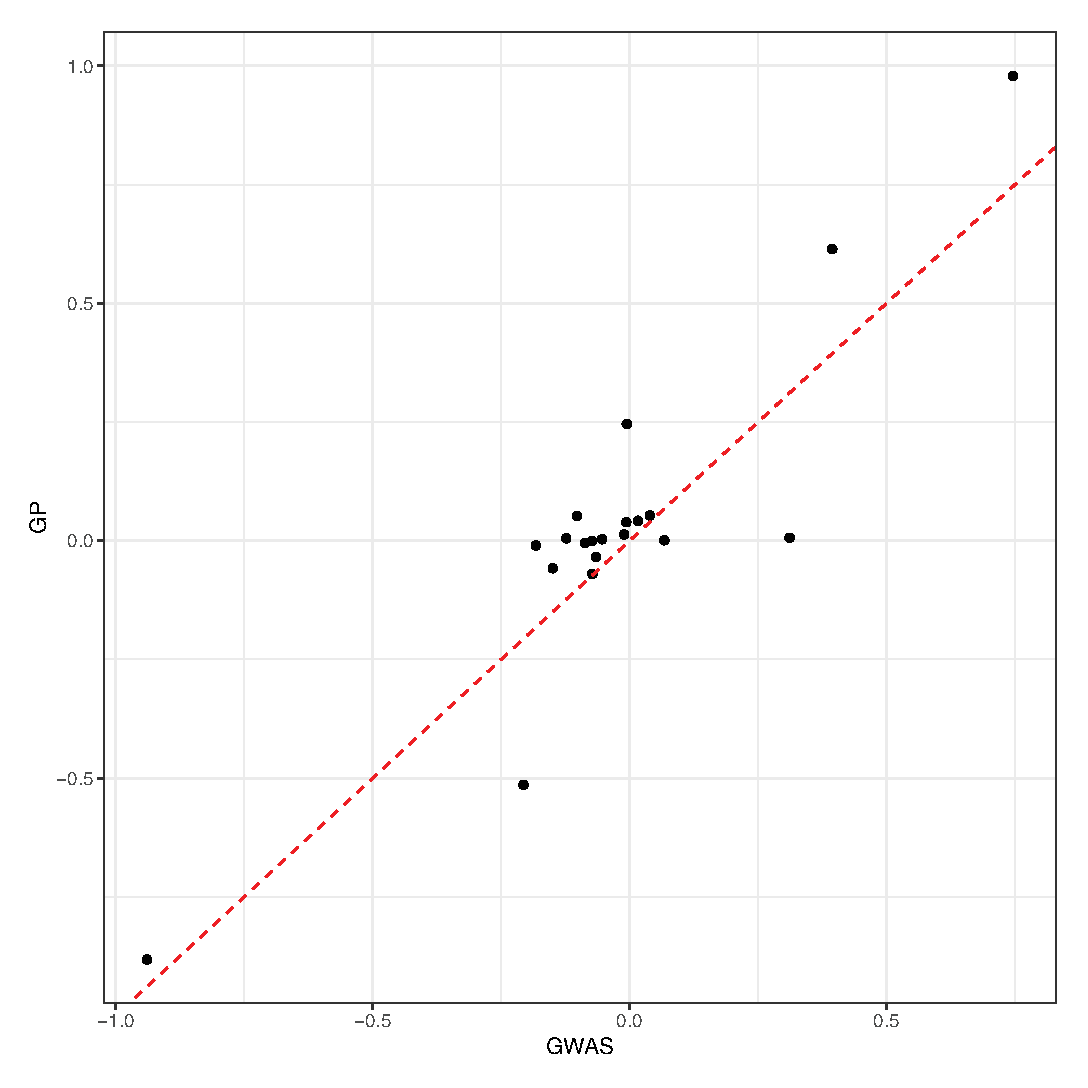
\includegraphics[width=10cm]{gwas-vs-gp.eps}
  \end{center}
  \caption{Estimated allelic effects from locus-by-locus GWAS (x-axis)
    and genomic prediction (y-axis).}\label{fig:gwas-vs-gp}
\end{figure}

More interesting than whether the estimated allelic effects are
similar is whether the predicted phenotypes are similar to the
observed phenotypes~(Figure~ref{fig:gwas-obs-vs-predicted}). As you
can see, in this simple simulated data set both approaches work
reasonably well, even though the estimated allelic effects are rather
different. In fact, the estimated mean squared error of the
locus-by-locus prediction is actually smaller than for the genomic
prediction~(6.02 vs. 8.02).

\begin{figure}
  \begin{center}
    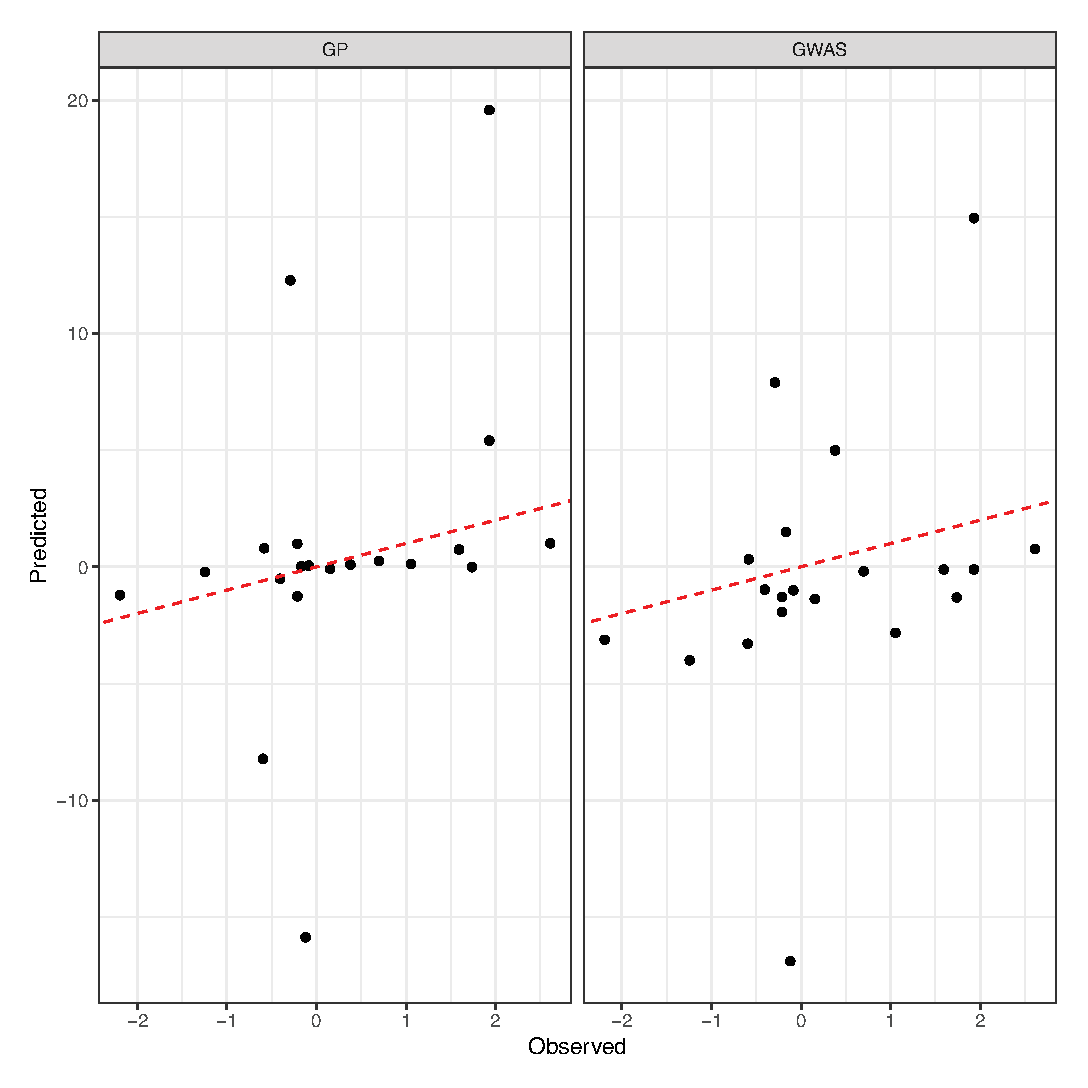
\includegraphics[width=10cm]{gwas-obs-vs-predicted.eps}
  \end{center}
  \caption{Predicted phenotypes {\it versus\/} observed phenotypes for
    locus-by-locus GWAS and genomic prediction.}\label{fig:gwas-obs-vs-predicted}
\end{figure}

